\documentclass[9pt,conference]{IEEEtran}
\usepackage{cite}
\usepackage{graphicx}
\usepackage{enumitem}
\usepackage{siunitx}
\usepackage{listings}

\def\BibTeX{{\rm B\kern-.05em{\sc i\kern-.025em b}\kern-.08em
    T\kern-.1667em\lower.7ex\hbox{E}\kern-.125emX}}
\begin{document}

\title{Novel Assistive Systems Applying Machine Vision and Human-Machine Interaction Technologies for Vulnerable Populations}

\author{\IEEEauthorblockN{Sidharth Shanmugam}
\IEEEauthorblockA{\textit{School of Physics, Engineering and Technology} \\
\textit{University of York}\\
York, England \\
ss2985@york.ac.uk}
}

\maketitle

\begin{abstract}
    This article investigates machine vision and human-machine interaction technologies to present two novel systems designed to assist vulnerable populations, encompassing older individuals, people with disabilities, and workers in treacherous conditions. A machine vision-based driver assistance system involving lane, driver's eye-gaze and blink tracking introduces an aid for workers in dangerous environments. Embodying human-machine interaction aspects into this system forms a novel design for cost-effective `railroad-style' autonomous transportation for older or disabled individuals. Discussions include technical analysis, safety and ethics considerations, and the potential impact on user livelihoods.
\end{abstract}

\begin{IEEEkeywords}
machine vision, human-machine interaction, lane detection, driver assistance, gaze detection, autonomous transport
\end{IEEEkeywords}

\section{Machine vision-based driver assistance system}
To gauge the driver's focus, a simple driver assistance system must track the vehicle's lane position and the driver's eye gaze and blinks. A vehicle's deviation from the centre of the lane, paired with repetitive blinks or an off-centred gaze in the driver's eyes, denotes extended fatigue or distraction of the driver. With the implementation of an alert system, which alerts not only the driver but other road users, this system can help workers in dangerous conditions, such as truck drivers traversing roads with narrow lanes and combatting fatigue. Abstracting into three fundamental mechanisms can drastically help with the development of this assistance system:

\begin{enumerate}[label=\alph*.]
    \item lane detection and tracking: detection of the lanes and calculating the distances from each side to track the average position of the vehicle.
    \item gaze detection and tracking: detecting and tracking the pupils of the driver's eyes to calculate the average time spent looking off-centre.
    \item blink detection and tracking: detection and tracking of blinking eyelids to calculate the average blinks or the average time of closed eyelids over some time.
\end{enumerate}

\subsection{Lane Detection and Tracking}

The lane departure warning system is quite a mature product, first unveiled in 1989 as a concept and working prototype fitted to the Rover SD1, but later debuted in 2000 as a production-ready system for the Mercedes Actros line of commercial trucks \cite{b1}. Given the safety benefits, lane departure systems have become a mandatory feature for all cars in the European Union as of 2022 \cite{b1}\cite{b2}. The most popular method for detecting lanes across the industry is to employ the Canny edge detection algorithm, The Hough Transform, and various principles of camera calibration, perspective transforms, and colour filtering to determine the lane line edges from a live feed \cite{b1}. Three stages contribute to the lane detection system \cite{b3}:

\begin{enumerate}[label=\alph*.]
    \item pre-processing: low-level image processing consisting of an image crop to reduce the region of interest for more efficient computing, grayscale conversion in preparation for Canny edge detection, and noise reduction techniques such as erosion, dilation and image soothing for more accurate detection.
    \item post-processing: implementation of Canny edge detection resides in this stage using the pre-processed frames to detect the discontinuous lane markings, which The Hough Transform connects into a continuous line.
    \item road lane modelling: computation to detect the left and right lane markings will utilise the continuous line output from the post-processing stage, establishing the positions of the lane boundaries to calculate the vehicle positioning within the lane to detect deviation.
\end{enumerate}

The Hough Transform provides a highly efficient method for detecting straight lines in images, even with noise and missing data \cite{b4}. The Hough Transform works by converting the image space into a parameter space called The Hough Space, and through this space, it is possible to detect geometric shapes by identifying patterns \cite{b5}. This ability of The Hough Transform to identify shapes makes it an ideal tool for detecting lane lines for a self-driving car \cite{b6}.

\subsubsection{Prototype for Lane Detection and Tracking}

Extracting individual image frames from a continuous video stream simplifies the logic of this system. The work in \cite{b3} forms a robust starting point for achieving a lane detection system. As the paper states, there is a cropping step in the pre-processing stage to reduce computational overheads by removing unnecessary parts of the input image. A single-channel conversion to grayscaling will reduce image data complexity to enable faster Canny edge detection. Although the mention of a noise reduction step in \cite{b3}, a detailed explanation nor a visual description is present, leading me to believe its exclusion in the proposed system. As the work in \cite{b7} discusses improvements in the Canny edge detection method by pre-processing the image by stretching the image histogram, the inclusion of a histogram equalisation step will occur post-grayscaling in this system. Inspired by the work in \cite{b6}, applying a Gaussian Blur filter ensures the disregard of as many false edges as possible by reducing noise and smoothening the image.

The work in \cite{b3} mentions, ``Canny edge detection is implemented in the post-processing stage'' But confusingly, later in the paper, a diagrammatical outline shows this step within the `pre-processing' stage. The Canny edge detection step will occur in the post-processing stage to avoid confusion and enhance stage separation. Despite applying an image crop, the Canny edge detection will still provide results outside the region of interest (ROI). Inspired by the work in \cite{b6}, cropping the Canny output to the triangular ROI will reduce additional computational overheads and improve The Hough Transform step. Finally, in the post-processing stage, The Hough Transform will generate continuous lines representing the lane marking detections, providing a foundation for lane tracking.

Overlaying The Hough Transform results over the image will provide a visualisation of the machine vision-based road lane marking detection helpful in gauging the system performance. Harnessing the fixed perspective characteristic of the system makes it possible to track vehicle lane positioning by measuring the x-axis location of the vertical base of the left/right lane lines. Veering towards the left lane can be denoted by an increase in the x-axis position of the left-hand lane line base, and veering towards the right can be denoted by a decrease in the x-axis position of the right-hand lane line base. Vehicular deviation from a lane is denoted by whether the base position of each lane line exceeds/falls from a fixed threshold x-axis position value. Threshold optimisation must happen before system implementation by accounting for the width of the vehicle and the perspective/positioning of the camera. Tracking the mid-point x-axis position of the automobile over time, normalising the value w.r.t. the lane positions, and then calculating the variance of this data can measure the driver's dispersion within the lane. This result forms the basis of the metric to gauge the driver's fatigue and focus levels, with a higher variance denoting high fatigue or low focus.

\begin{figure}[htbp]
    \centerline{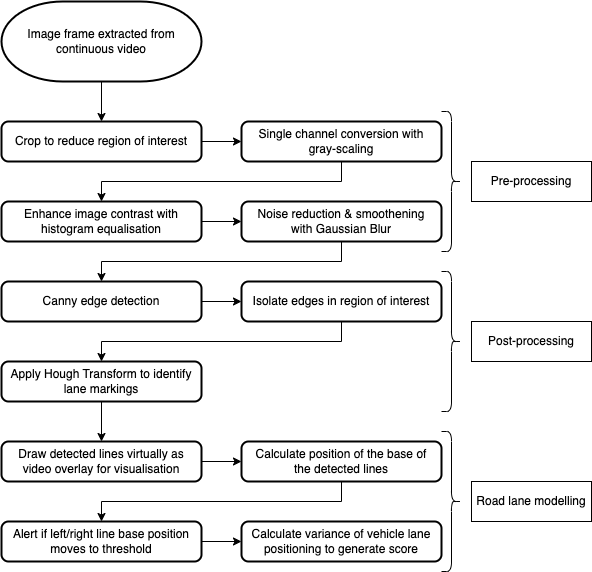
\includegraphics[width=0.5\textwidth]{assets/lane-detection-flow.png}}
    \caption{Flow of lane detection and tracking logic.}
    \label{f1}
\end{figure}

The developed software, source code in Appendix \ref{a1}, utilises the Python (3.11.2) programming language and employs the OpenCV library to access highly optimised and efficient computer vision algorithms, reducing development overheads tremendously. The software incorporates a cropping stage before processing the frame to ensure compatibility with a wide range of input video dimensions. A constant definition for the height and width of the input video feed is present, which the initial crop utilises for generating a window aligned at the bottom of the original frame and horizontally centred, ensuring a 640(w)x480(h) crop (dimensions as defined by the constants) for any higher resolution video feed. This cropping is merely for input video dimension standardisation, and regions outside of the ROI will still be present to ensure easy data visualisation. A YouTube video \cite{b8} forms the perfect testing input for this system, consisting of an almost 4-hour video feed of a nighttime drive from Busan to Seoul through various types of roads and lighting conditions.

\begin{figure}[htbp]
    \centerline{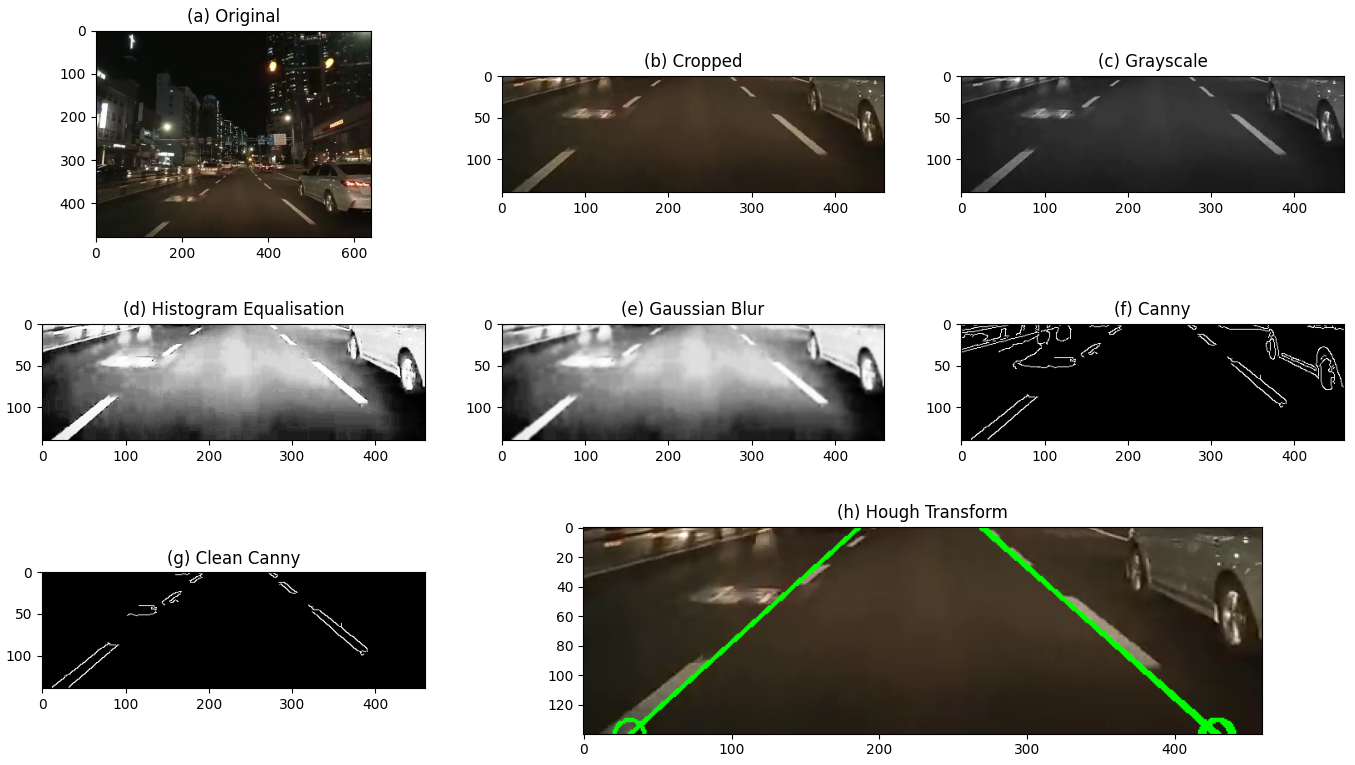
\includegraphics[width=0.5\textwidth]{assets/LDS_plot.png}}
    \caption{Stage-by-stage plots of the lande detection and tracking system outputs. Original frame shown in (a) which is then cropped in (b), grayscaling filter applied in (c), with histogram equalisation in (d) and a Gaussian blur in (e), output from the Canny edge detector in (f), with results cropped and shown in (g), the road lane markings identified by The Hough Transform are overlayed on to the frame in (h).}
    \label{f2}
\end{figure}

After the input video feed standardisation to 640x480, the first step in the pre-processing stage is an additional frame crop to reduce the ROI. Using the matplotlib Python library, a plot of the normalised video with the axis labels can help choose the lane width with the lane markings and how far forward the system needs to see. With the ROI region coded as shown in Figure \ref{f2}, grayscaling occurs to reduce computational complexity by converting to a single-channel image. The application of histogram equalisation, then a Gaussian blue filter, prepares the frame for the post-processing stage of the system.

Implementing a zero-parameter automatic Canny edge detection logic simplifies the system greatly \cite{b9}. Though not truly a `zero-parameter' due to the necessity of a threshold `sigma' parameter, it vastly simplifies logic using statistical offsets, enabling single parameter tweaking for optimisation. A further crop with an isosceles trapezoid-shaped masking window on the Canny algorithm output eliminates all edge information outside the lane markings, further isolating the ROI. The clean Canny output enables a more efficiently performed Hough Transform to detect the road lane markings. The Hough Transform implementation has further logic to ensure only lines within a specified diagonal angle range are output from the step to ensure only lane markings are detected. The definition of programmatical constants for the angle range values enables simple optimisation. The Hough Transform generated lines drastically extend the frame size due to the presence of a multiplier as per the OpenCV tutorial documentation \cite{b10}. Modifications to The Hough Transform logic in this lane assist implementation include scaling the detected and drawn lines to fit within the border of the image frame. Programmatical detection of road lane markings consists of parsing the start and end coordinates of the detected lines. The Hough Transform generates two coordinate points for each detected line, with a starting point at the bottom of a positive gradient line and at the top of a negative gradient line. More simply, starting points will be on the left and ending points on the right.

Left-hand lane markings will start at a y-axis value equal to the frame height and finish at a y-axis value equal to 0, with arbitrary x-axis values. Right-hand lane markings begin at the top and end at the bottom of the frame, with arbitrary x-axis values. This understanding makes it easier to differentiate between the two sides of lane markings and to parse the position of the base of each line. The departure warning implementation will use the base positions of each lane marking, alerting once each position passes an x-axis threshold (programmatically defined as a constant). Shown in Figure \ref{f2} is the implementation in action with lane detections shown in green and the bases of each also circled in green. When the driver approaches too closely to either lane, the lines will turn red, alerting a lane departure. The vehicle lane tracking implementation collects the base location of left-hand and right-hand lane markings, using linear interpolation for intermediate predictions for frames with undetected lane markings. The centre point between the two lane markings is the vehicle's position. Calculating the driver's lane position variance (LPV) metric, showing the variance in the vehicle's position w.r.t. the lane markings, is possible using an array of vehicle positions. Including garbage collection to limit the maximum and minimum number of collected vehicle position data by deleting old data once passing the maximum threshold prevents a gradual slow-down of the program due to a massively growing array.

\begin{figure}[htbp]
    \centerline{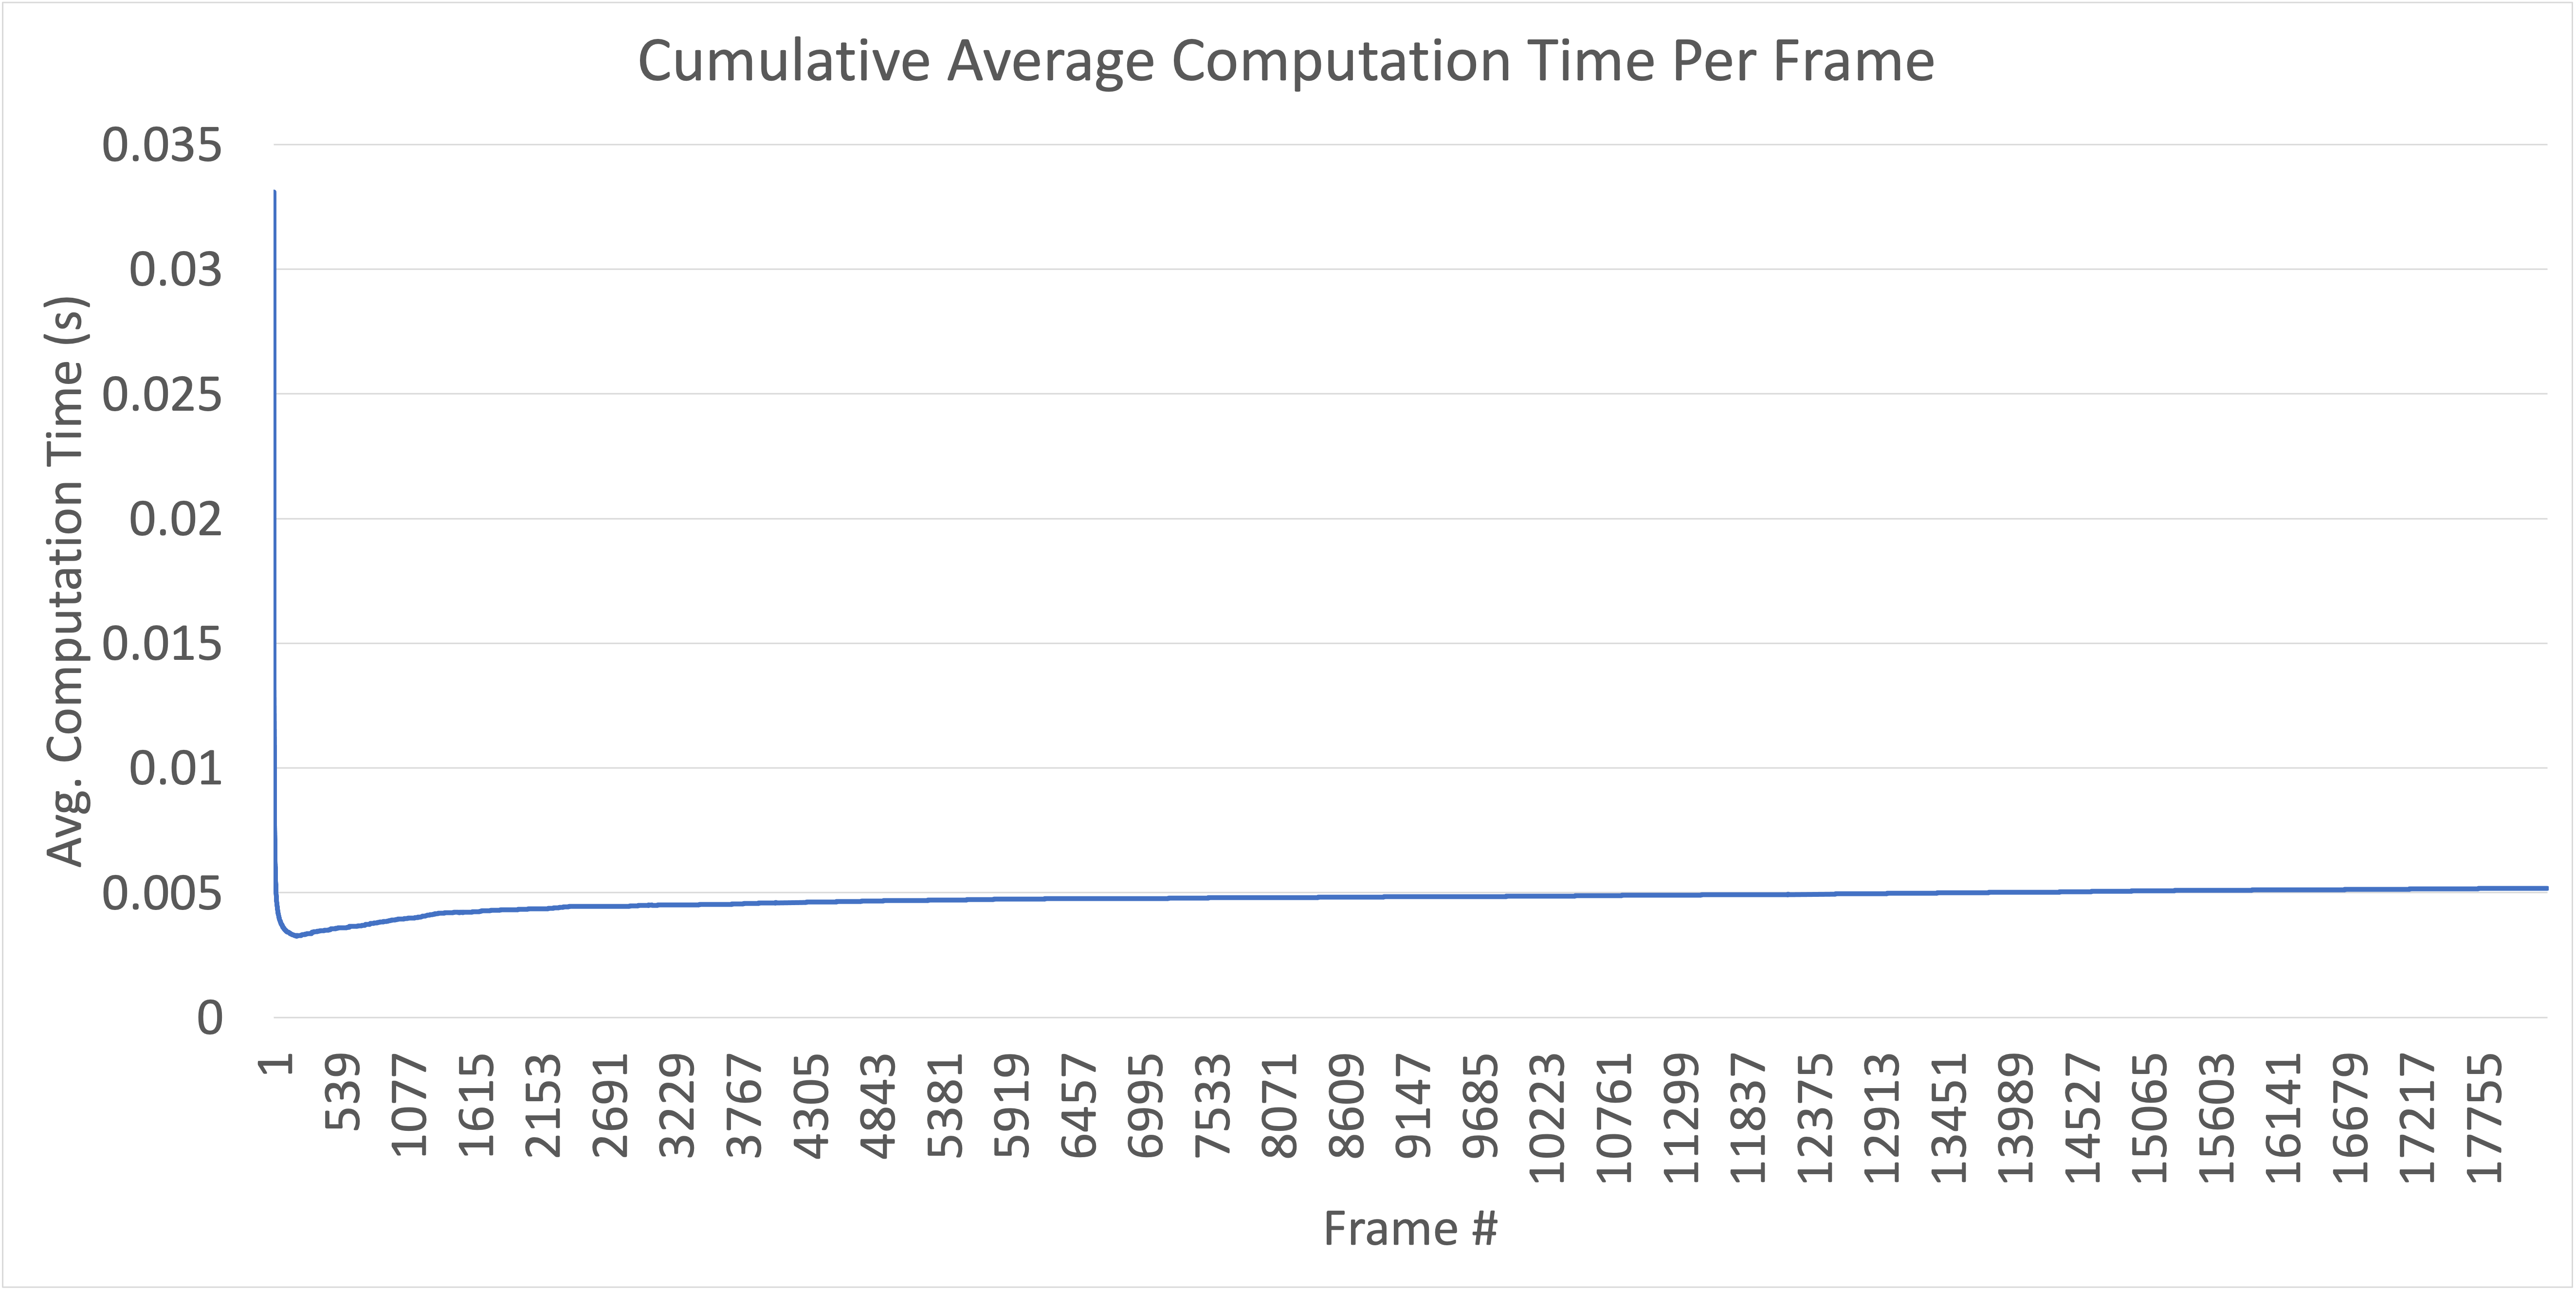
\includegraphics[width=0.5\textwidth]{assets/LD_Avg-FPT.png}}
    \caption{Cumulative average of the time taken to compute each frame for lane detection and tracking.}
    \label{f3}
\end{figure}

\begin{figure}[htbp]
    \centerline{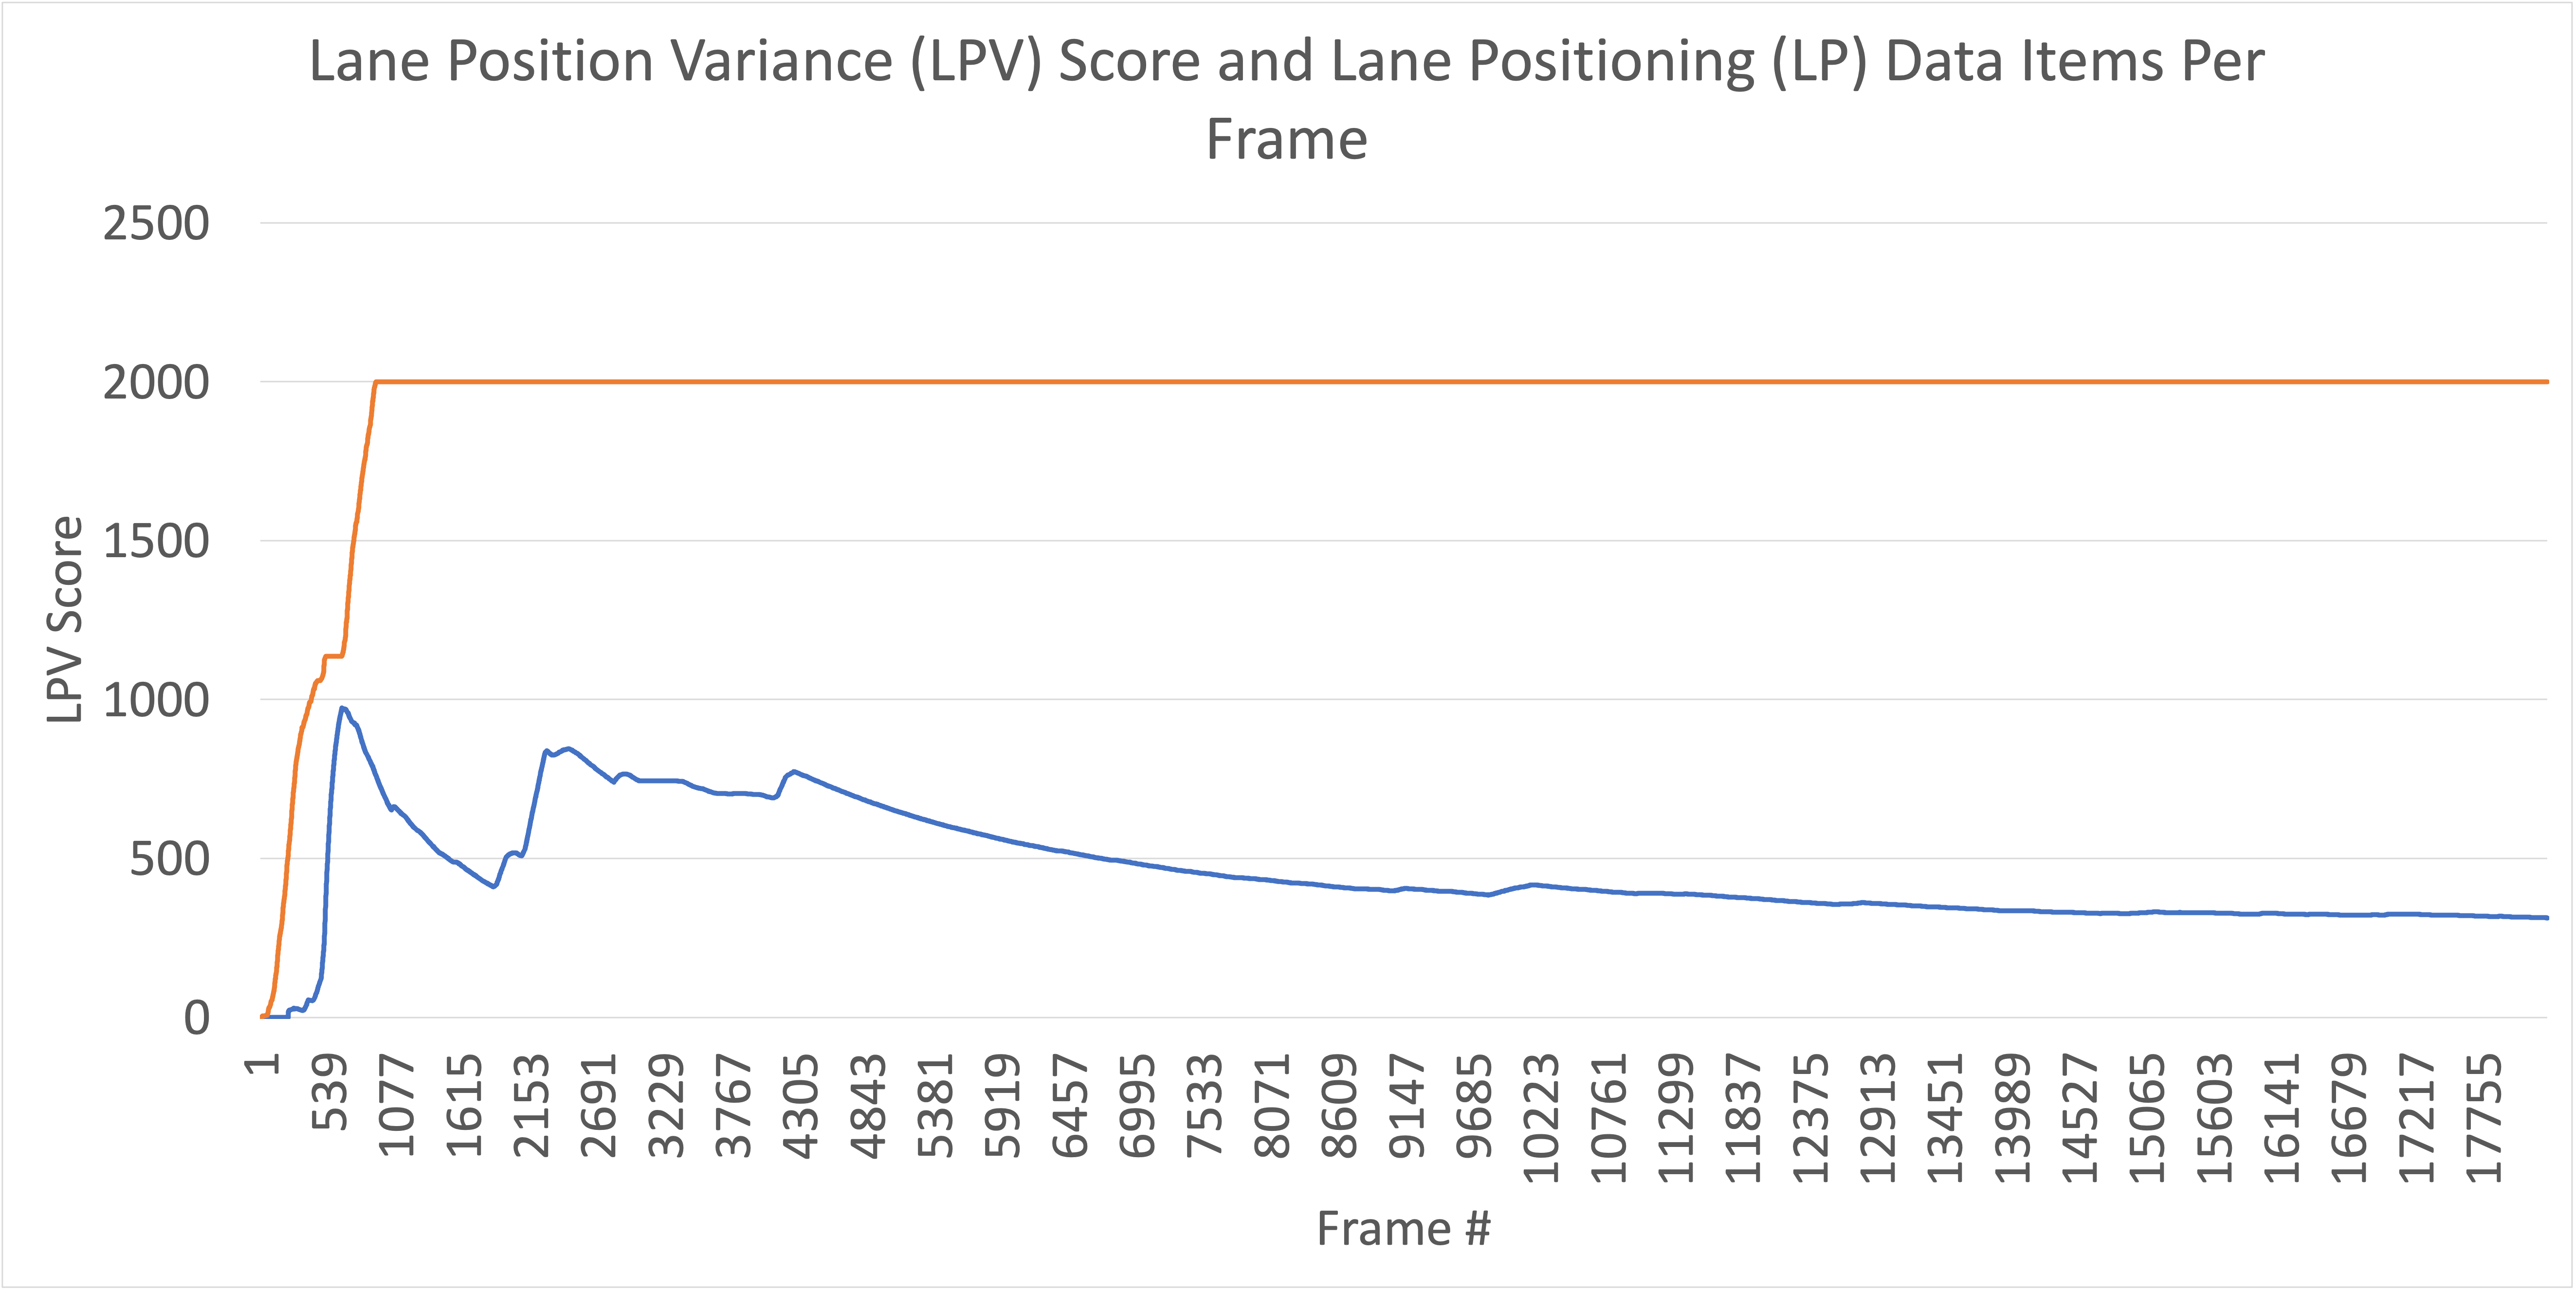
\includegraphics[width=0.5\textwidth]{assets/LD_Avg-LPV.png}}
    \caption{(Blue trace) cumulative average of the LPV score at each frame for lane detection and tracking, calculated using the footage between 0:18-13:00 from the testing video \cite{b8}. (Orange trace) number of lane positioning data items used to compute LPV score.}
    \label{f4}
\end{figure}

The mission-critical essence of this system permeates from its fundamental requirement of detecting and alerting hazards as they occur. The processing time for each frame must be as low as possible to ensure the software can keep up with the input video feed. The system implements start and finish timestamping to acquire metrics for real-time performance. The YouTube video as before \cite{b8} but only including the footage between 0:18 and 13:00 forms the basis of these real-time metrics plots in Figure \ref{f3} and Figure \ref{f4}. Shown in Figure \ref{f3} is the cumulative average for the time taken to compute each frame. We can see an average frame compute time of \SI{5.2}{\micro\second}, resulting in an average of roughly 192 frames per second. It is unclear what caused the tremendous spike in compute time during the first frame, but I assume this to be OpenCV-related, resulting from populating GUI windows for the first time.

Shown in Figure \ref{f4} is a plot of the lane position variance, a score calculated from the cumulative average of the variance in the vehicle's position w.r.t. the lane markings from each frame. The spikes in this score at the beginning of the footage are due to the driver making multiple lane changes and swaying within the lane. However, once the driver enters the motorway, the score starts to settle down, a result of fewer to no lane changes and swaying. The graph also has an overlayed plot of the number of lane positioning data items, a count of the total number of left-hand and right-hand lane base positions. To ensure as much interpolation accuracy as possible, the calculation of the LPV score only starts when there is a minimum of 500 previously recorded lane marking positions. The higher the amount of lane position data points, the slower the linear interpolation algorithm will be. The system's effort to maintain a maximum of 2000 points to ensure performance is visible as the graph plateaus at this value.

\subsection{Blink and Gaze Detection and Tracking}

Although separating blink and gaze aspects into individual blocks helps with conceptualising the system, in implementation, it is much easier and more efficient to merge them into a single block. The first driver monitoring implementation was introduced by Toyota in 2006 for its and Lexus' latest models, incorporating face tracking using IR LED detectors and CCD cameras \cite{b11}. Although 18 years have passed since then, only a handful of car manufacturers have adopted this technology, including BMW, Ford, Cadillac, NIO, XPeng, and Mercedes-Benz, incorporating this technology in some of their models. Albeit regulated, this technology is not yet mandatory as per the European Union \cite{b12}, which could be the primary cause for this lacklustre adoption. As a result, there is no industry-standard methodology for this system. This system follows the same three-stage abstraction as the lane detection and tracking flow. The pre-processing stage is identical. The post-processing now includes Dlib machine learning-based functions \cite{b13} to detect faces and predict facial landmark coordinates, utilising Dlib's pre-trained 68-point facial model \cite{b14}. Finally, a binary inversion threshold filter before a Simple Blob Detection step facilitates pupil/iris detection. The final stage consists of driver monitoring logic, where results computation from the pre and post-processing stages occur to calculate the driver's fatigue and focus levels.

\begin{figure}[htbp]
    \centerline{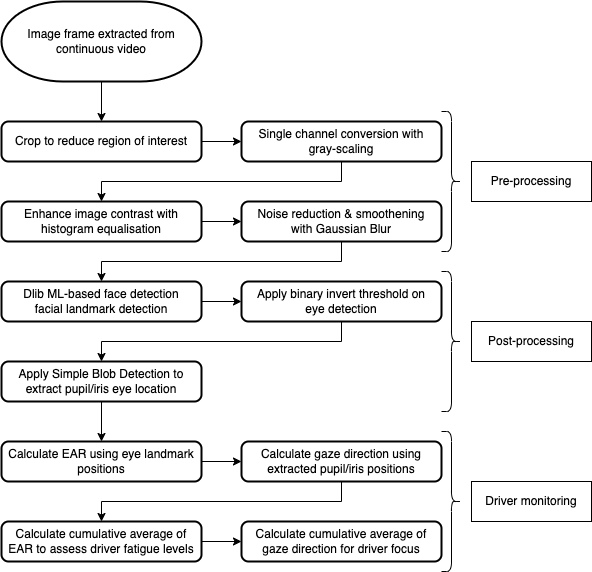
\includegraphics[width=0.5\textwidth]{assets/eye-detection-flow.png}}
    \caption{Flow of eye blink and gaze detection and tracking logic.}
    \label{f5}
\end{figure}

\subsubsection{Prototype for Gaze and Blink Detection and Tracking}

Following a similar approach to \cite{b15}, the programmatical implementation for this system, source code in Appendix \ref{a2}, uses a similar logic from the lane detection and tracking implementation. A crop is present to reduce the resolution of the feed to 640x480, programmatically defined as a constant, to speed up frame processing time. Grayscaling, histogram equalising and Gaussian filtering steps are present to improve system efficiency for detection and processing time, in addition to drastically enhancing the low light capabilities of this system. The detection of faces and facial landmarks is possible using the Dlib detection function with the trained 68-point landmark model. The eye aspect ratio (EAR) enables the detection of blinks by deriving from the positions of detected eye landmarks using the dimensions of the left and right eyes. The system calculates a cumulative average EAR over a fixed amount of time to form the driver tiredness score, currently set to a 600 frame sample size, which equates to 10 minutes for a 30 FPS input. The implementation alerts if the tiredness score drops below a certain threshold, notifying the driver that most of the 10-minute sample size consists of shut or near-shut eyelids.

Isolating each eye as a window is possible since landmarking accurately identifies each eye's coordinate bounds. With each isolated eye, applying a binary threshold allows for a clear separation between the pupils/iris and the sclera, forming an ideal preparation for the OpenCV Simple Blob Detection algorithm \cite{b16}. The initialisation of the Simple Blob Detector consists of deactivating the thresholding stage since the implementation already grayscales the frame. Filtering by colour is enabled, correctly setting the thresholded colour of the pupils/iris. Filtering by area is enabled since testing revealed that the dark spots of the pupils/iris take up most of the space in the frame.

\begin{figure}[htbp]
    \centerline{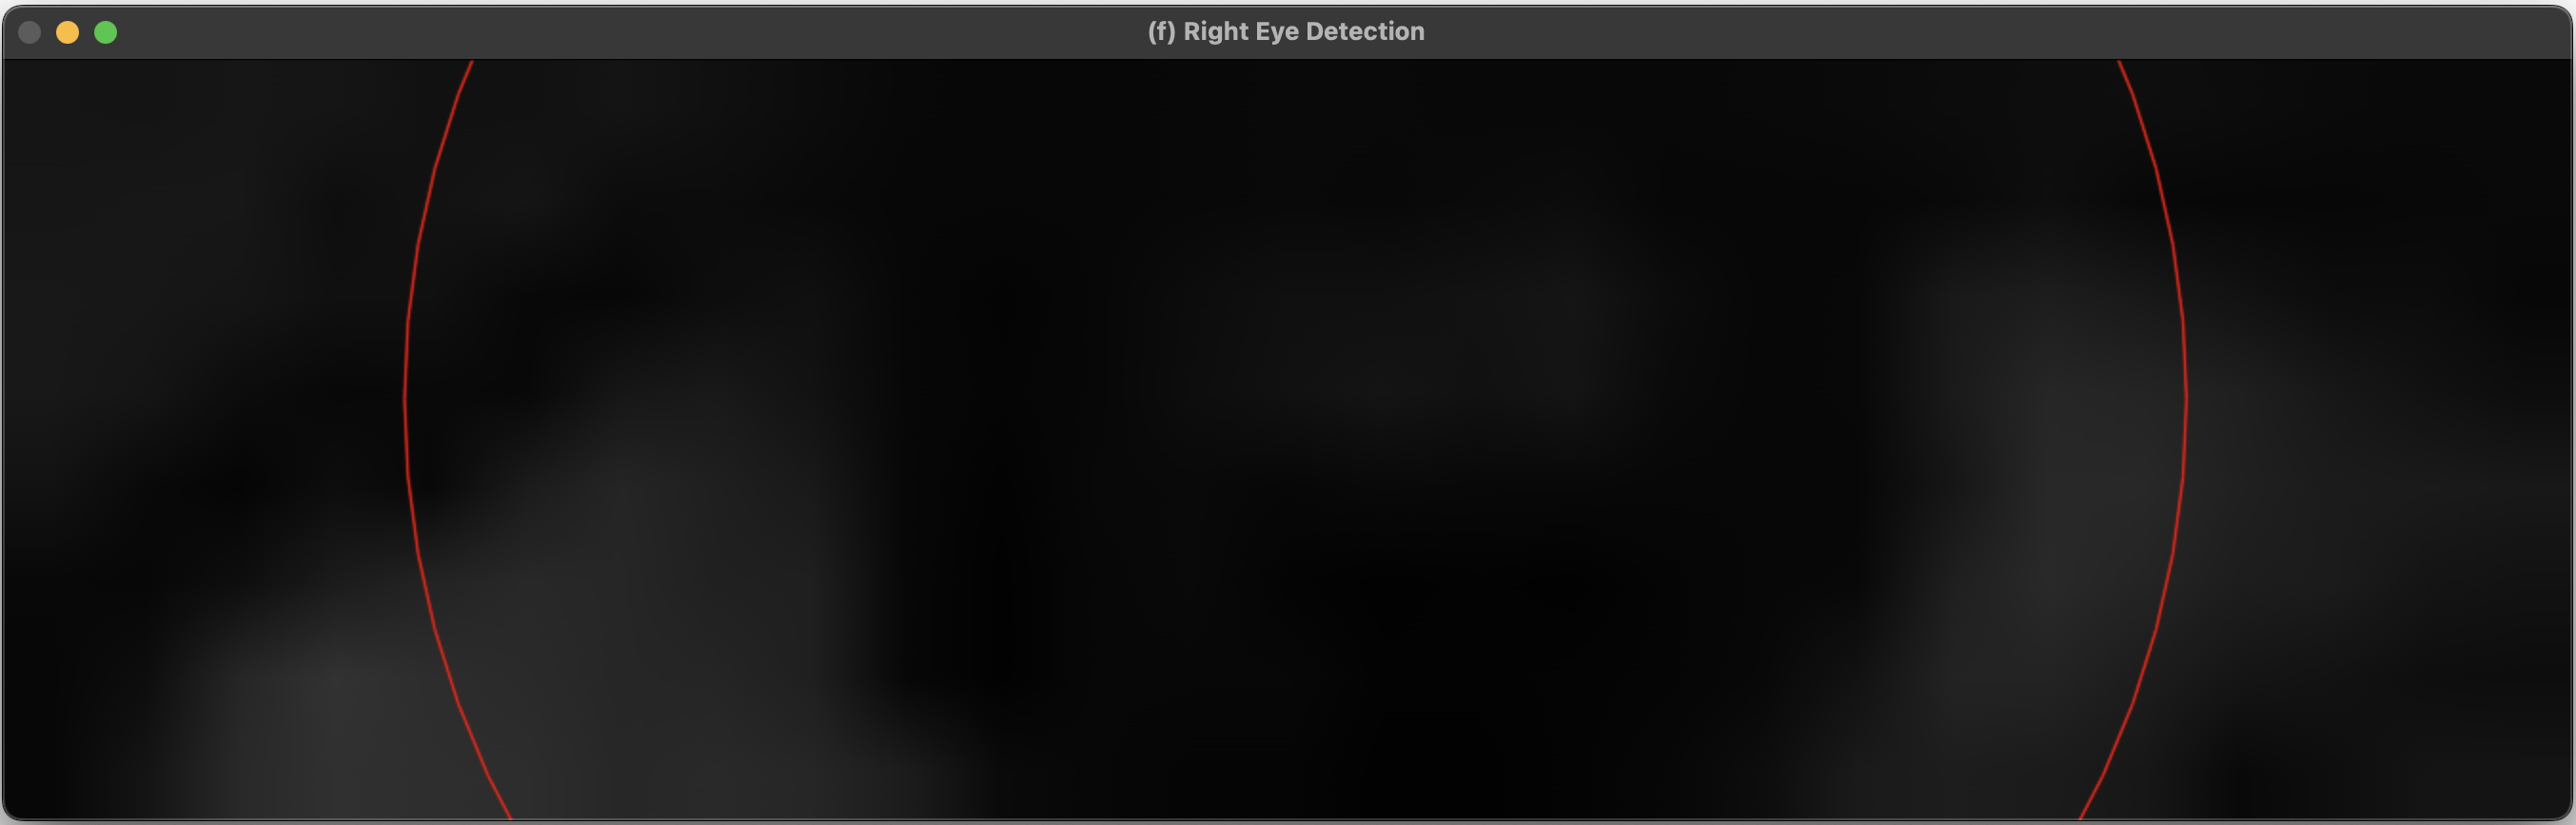
\includegraphics[width=0.5\textwidth]{assets/gaze-detection.png}}
    \caption{Visualisation of pupil/iris detection using the Simple Blob Detector for the gaze tracking system.}
    \label{f6}
\end{figure}

\begin{figure}[htbp]
    \centerline{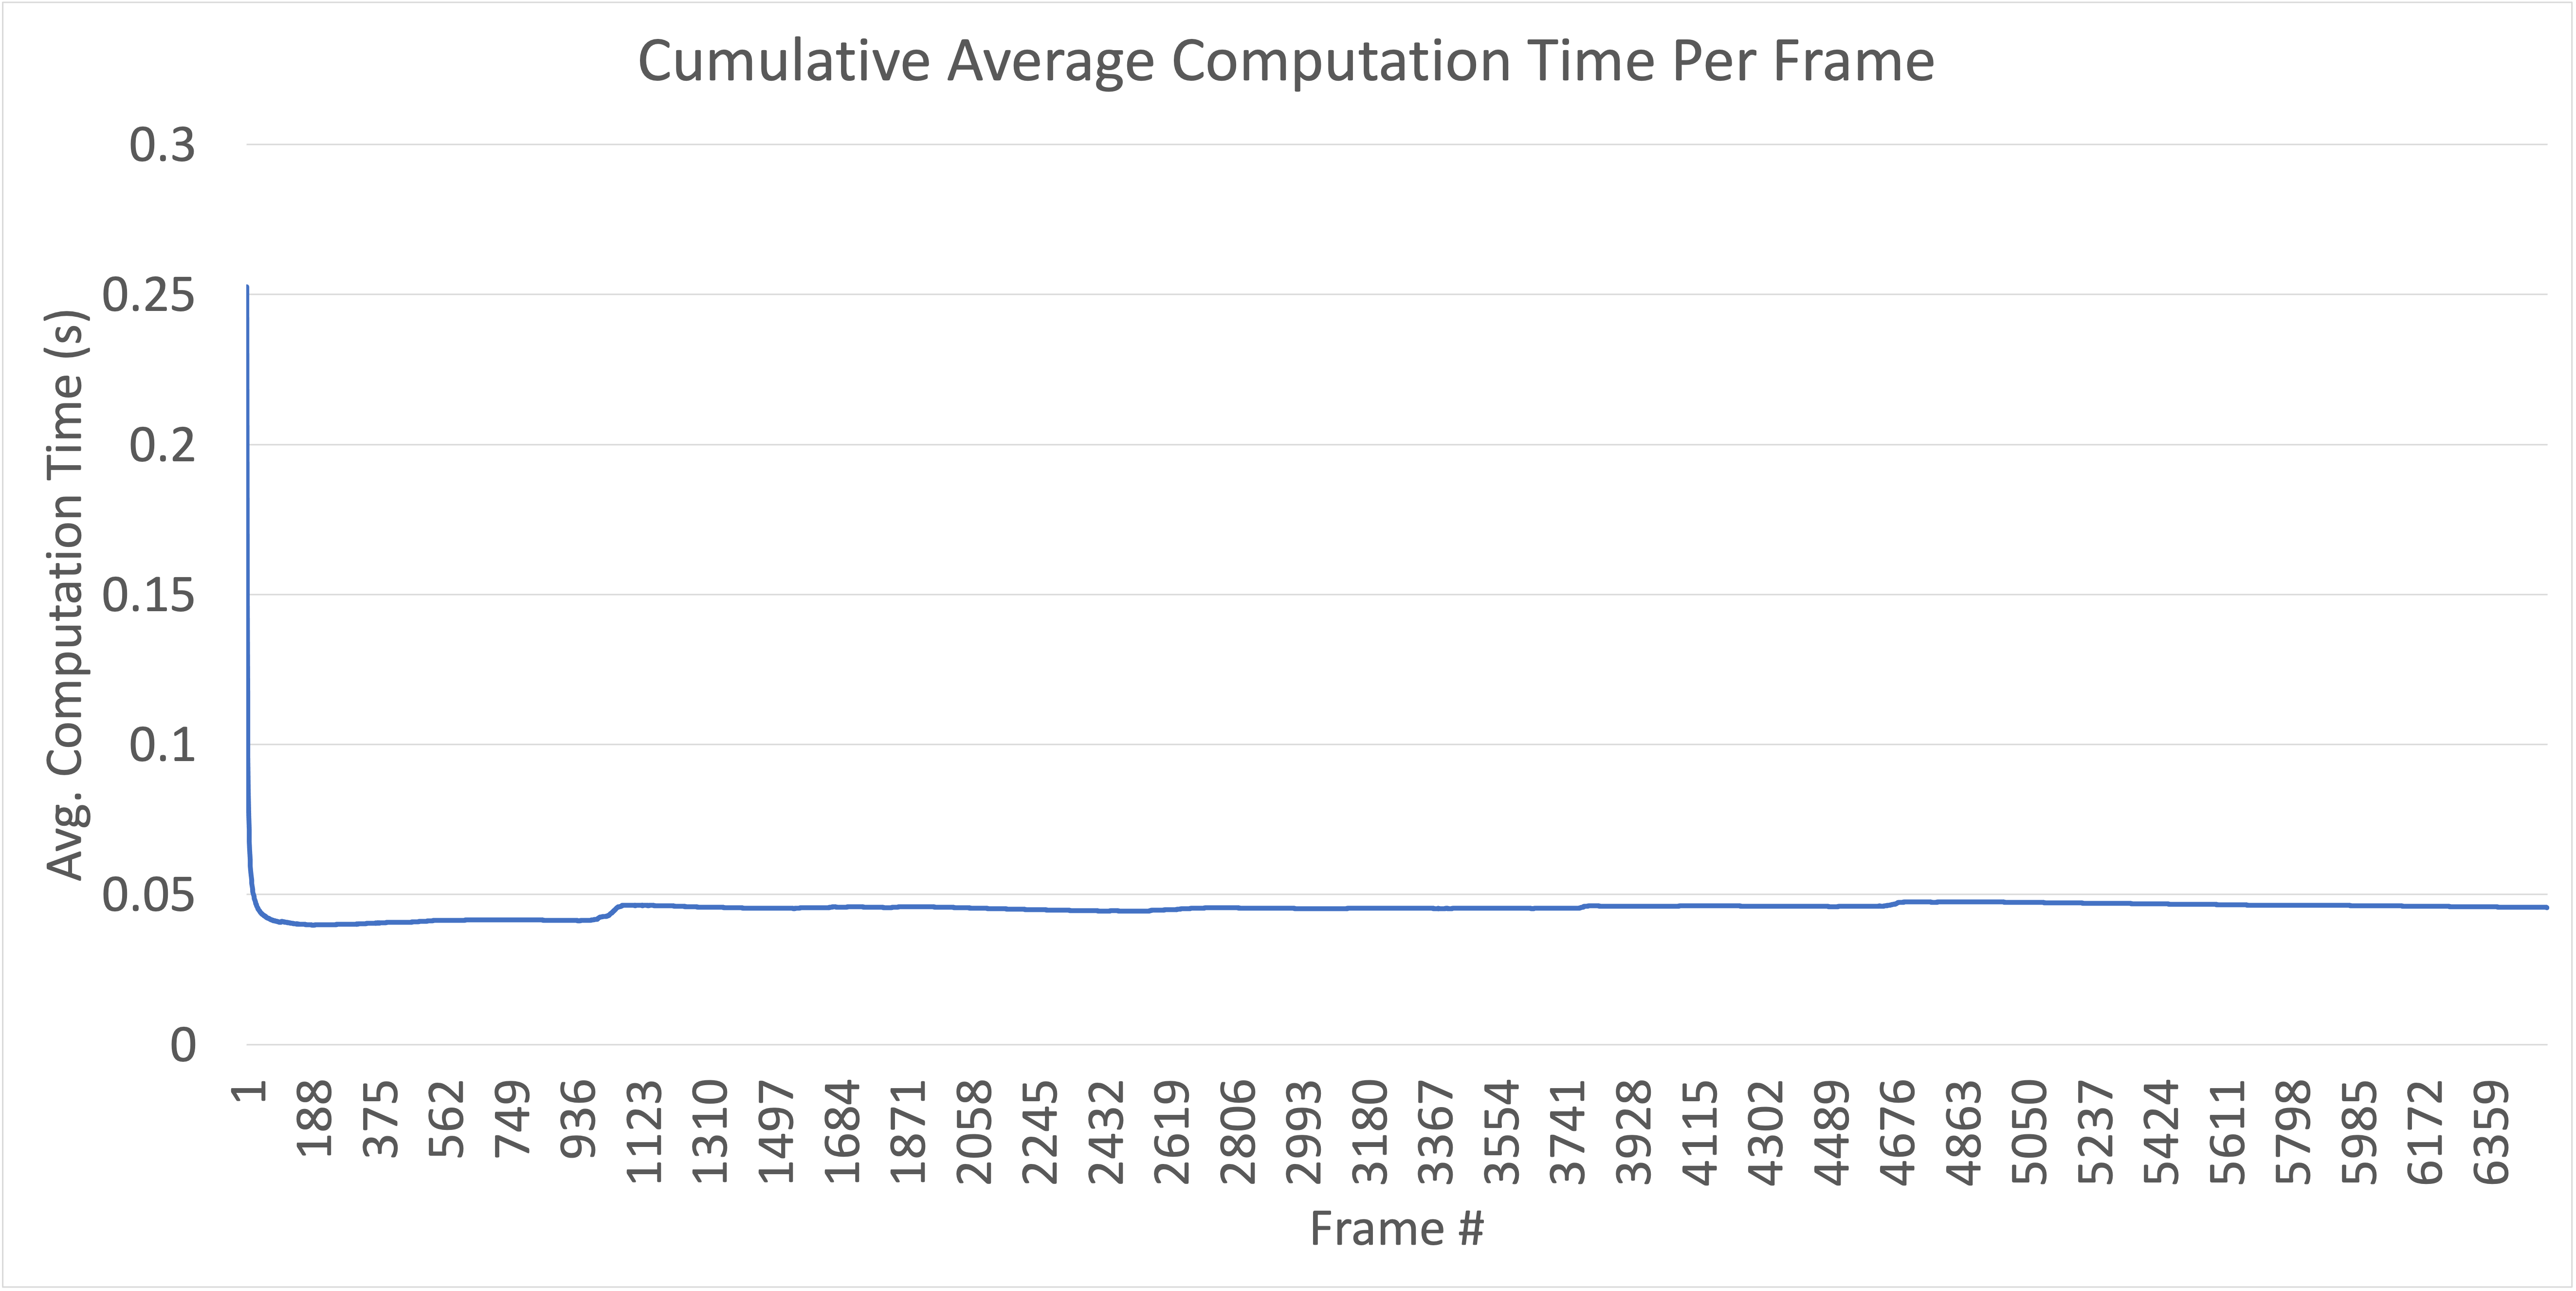
\includegraphics[width=0.5\textwidth]{assets/Eye_Avg-FPT.png}}
    \caption{Cumulative average of the time taken to compute each frame for eye detection and tracking.}
    \label{f7}
\end{figure}

Figure \ref{f6} shows the result of the blob detection, detecting the iris successfully. Though quite reliable at tracking left and right gaze directions, a paramount downside is that it does not track up and down movements competently, as the blob detection fails to detect. Tracking all gaze locations is crucial for a driver monitoring system. Workarounds are present, such as measuring the time the driver spends looking straight, left, or right since tracking this is comparatively reliable, then inverting this to generate the time the driver spends not looking ahead, allowing a gauge on the driver's focus. Despite lacking gaze tracking functionality, Figure \ref{f7} shows an average \SI{45}{\micro\second} frame compute time, with the same spike in the first frame, just like the lane detection and tracking system. The average frame compute time value exhibits an approximate 25 frames per second compute rate for this system, only a five frames per second difference from my webcam capture rate.

\begin{figure}[htbp]
    \centerline{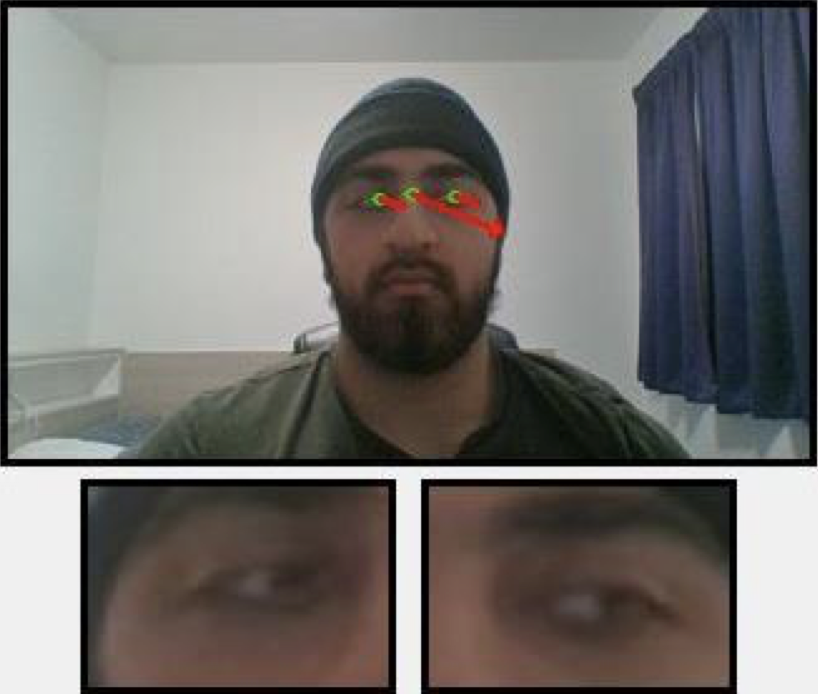
\includegraphics[width=0.5\textwidth]{assets/Gagan-eye.png}}
    \caption{Eye gaze and blink tracking demonstration of a different system [18].}
    \label{f8}
\end{figure}

Unlike the lane detection and tracking system, a highly efficient frame computing capability is not a necessity for this system. Due to its reduced mission criticality, the fundamental goal would instead be to focus on highly accurate gaze tracking. The work in \cite{b17} implements a Regression Convolutional Neural Network on top of the facial landmark detection to track eye gaze. Initialising and running the Python code associated with this paper, located in a GitHub repository \cite{b18}, reveals a veraciously impeccable gaze detection implementation achieved by accelerating traditional machine-vision methodologies using machine-learning techniques, shown in Figure \ref{f8}. The improved tracking accuracy comes at a price of performance, but this substantial drop in frame rates is a sacrifice to gain reliable measurements.

\subsection{Implementation of System}

Interlinking the lane detection and tracking system with the blink and gaze detection and tracking implementation assembles the complete driver assistance solution. Computing an overall score using the LPV and tiredness/focus score from the two individual systems is possible and can gauge the driving safety score for the driver. The prospect of employing several interaction modalities can improve the safety of the driver and surrounding traffic:

\begin{enumerate}[label=\alph*.]
    \item Visual feedback: A visualisation of the detected lane markings coloured to portray lane departure can be overlayed on a video feed, perhaps augmented via a heads-up display, providing assistance to maintain centred lane positioning. Alerts to show in the instrument cluster or heads-up display when the driver struggles to maintain centre position (LPV score above threshold), when the driver's blinking is more frequent (tiredness score via blink tracking above threshold), or when the driver's focus is low (focus score via gaze tracking below threshold). External car lighting can alert the driver and surrounding traffic by implementing a similar design as Audi \cite{b19} by integrating results from this driver assistance system. Matrix LED headlight technology draws symbols on the road to emphasise lane markings, with warning triangles and concentrated light flashes to warn the driver and surrounding traffic and organic LED taillights to provide visual information to surrounding traffic.
    \item Auditory feedback: Employing spacial audio cues for lane departure warnings, developed in a way where the audio direction comes from the side of the lane departure, forms the ultimate warning system. It's not necessarily noise that keeps you awake - it's the sudden change in noise that's most likely to wake you up \cite{b20}. Harnessing this ideology can administer a prime solution to combat driver fatigue; playing a loud sporadic noise, such as a dog barking at random intervals when the tiredness score surpasses a certain threshold, can help wake the driver. A more ordinary solution is to display an alert on the instrument cluster or a heads-up display to suggest the driver take a coffee break.
    \item Haptic feedback: Vibrations or physical movements of the steering wheel can alert the driver of lane departure. Since the system knows the lane positioning, it can take a further step by applying steering inputs to ensure the vehicle maintains a centred position within the lane. Implementation of seat vibrations can enhance the alert system, especially in the case where the driver is asleep or unconscious with both hands off the steering wheel. A more aggressive seat jolt, implemented in the same fashion as the load sporadic dog barking, can wake the driver more efficiently.
    \item Climatory feedback: Upon driver fatigue detection, the driver assistance system can autonomously set the car's climate to an unbearably cold cabin temperature, catalysing an unpleasant thermal environment to wake the driver. Some car manufacturers, such as BMW \cite{b21}, have implemented climate-control-based cabin scent diffusers, crafting a perfect method to wake the driver when fatigued by filling the cabin with citrus, coffee, or similar aromatherapeutic scents to stimulate the brain \cite{b22}.
\end{enumerate}


\subsection{Safety, Ethics, and Impact of System}

Statistics show that a lane assist system results in an 11\% reduction in crashes of all severities and a 21\% reduction in crashes with injuries, with results suggesting the saving of thousands of lives each year if every passenger vehicle in the US implements a lane departure warning system \cite{b23}. Studies show that human error, including fatigue or drowsiness, contributes to 80.6\% of road accidents \cite{b24}, with reports stating that 54\% of adult drivers feel drowsy while driving and 28\% attesting that they fall asleep while driving \cite{b25}, the need for a reliable driver fatigue detection and monitoring system, which alerts the driver has never been more imperative as our reliance on vehicles has exponentially increased, leading to higher levels of road users.

Despite the high praise for driver assistance technologies, a voluminous risk still exists involving the shift of trust to machine vision and computer algorithms to perform safety-critical decisions. For example, false lane detection alerts can potentially startle the driver and lead them to perform unsafe manoeuvres to mitigate a risk that was never present. Moreover, the driver monitoring system responsible for tracking driver docus and fatigue, when implemented into driving trackers (black-box trackers) for car insurance policies, can result in adverse insurance premium changes due to false results. Strategies to improve system performance for enhanced environment tracking are present, though a computer vision approach can never be perfect due to varying environmental conditions. A key factor to mitigate the risk is considering these systems as a helping hand and not holding predominant trust in them. Another aspect to consider is privacy and ethicality, especially with the constant recording of surrounding roads and the driver's face to ensure system functionality. Employment of edge computing, ensuring all data processing occurs within the vehicle, can mitigate privacy risks by preventing data transfer to servers. However, this can drastically bottleneck the system performance as power-limited and smaller form factor computers inside vehicles replace the powerful and centralised server farms.

70\% of survey respondents believe that in-vehicle Driver Monitoring Systems can improve road safety and help reduce accidents caused by distracted or fatigued drivers, with only 28\% of UK consumers knowing this new technology \cite{b26}. Carmakers and regulators must strive for widespread adoption, to raise awareness, and to improve road safety for all.

\section{Human-machine interaction-based autonomous transportation system.}

In the amalgam of daily activities, there exists a spectrum of challenges, often unseen by the vast majority, that inhibit the lives of older individuals and those living with disabilities. From elementary tasks of dressing, bathing, feeding, and moving between spaces to the broader aspect of travelling independently, all pose hurdles, wielding a power to erode independence, strip away dignity, and confine individuals. In light of these challenges, integrating machine vision and human-machine interaction technologies emerges as viable solutions. Acting as a beacon of hope, leveraging these innovative technologies brings the potential to support vulnerable populations in their day-to-day lives. By extending the scope of machine vision applications, these systems can offer a transformative shift to ease the burdens and hurdles encountered in their routines.

The importance of such assistive systems embodies a promise to transform lives, drastically increasing the quality of life for many. Beyond the improvement of convenience, these systems represent a gateway to boost independence, bringing the joy and fulfilment of engaging in more activities. This second part of the article explores an autonomous transportation system, extending from the machine vision technologies explored previously and the fusion with machine vision methodologies, conceptualising an advanced assistive system seeking to redefine mobility for vulnerable populations. This novel approach aims to materialise as a mobility aid that transcends barriers in transportation, offering seamless navigation within large buildings such as supermarkets and hospitals.

\subsection{Design Analysis}

Large buildings, bustling with activity and often maze-like in structure and layout, pose substantial challenges for the vulnerable population traversing these spaces. Supermarkets, hospitals, and similar expansive structures designed to accommodate multitudes of people and diverse functionality have become labyrinthine for individuals with mobility limitations. The two main challenges are the following:

\begin{enumerate}[label=\alph*.]
    \item Navigational: The sheer expanse of these buildings can pose a significant hurdle, with lengthy corridors, multiple floors, and complex layouts, often extremely confusing to all, not just the vulnerable populations. The struggle to find specific sections within these structures, aisles in a supermarket or wards in a hospital, for example, can lead to immense frustration and exhaustion.
    \item Physical: Narrow passages, crowded areas, and high shelves in supermarkets can impede smooth movement. In hospitals, intricate floorplans, diverse elevations, and obstacles generated by unexpected medical equipment placement can add further complexity, hindering comfortable navigation and travel for vulnerable populations.
\end{enumerate}

The characterisation of challenges aids the conception of the system requirements for this autonomous transportation system. For the development of a system that provides effective aid to the vulnerable population in navigating these expansive and challenging environments, several critical considerations and requirements emerge:

\begin{enumerate}[label=\alph*.]
    \item Intuitiveness: Simplicity and straightforward guidance are paramount for vulnerable populations. The system must be intuitive, offering clear and accessible directions, incorporating visual and auditory cues aligned with clarity, and minimising confusion and cognitive overload. Intuitive UI, with readable fonts, icons, and a pleasant colour scheme, is critical as vulnerable populations may not have experience with complex technological systems.
    \item Adaptability: The system should possess the ability to adapt, catering to the diverse layouts and structures of different buildings. Whether in a hospital, supermarket, or any other expansive structure, the system must seamlessly and precisely accommodate various floor plans and spatial intricacies, such as crowds, hazards, and obstacles.
    \item Real-time: In vastly changing environmental conditions, accurate real-time updates are crucial. The system must factor the efficiency of frame processing times to ensure system actions are instant without a large delta to the environment. Similar to the lane detection and tracking system, it's imperative to action dangers such as path deviation of the transportation system or the detection of newly spawned hazards as soon as possible.
    \item Accessibility: Incorporating accessibility features is essential when developing a system that wholly encompasses the vulnerable population. The system should accommodate users with different mobility and sensory abilities, implementing functionality such as voice-guided navigation, tactile interfaces, or eye tracking to ensure inclusivity.
    \item Safety: Similar to real-time requirements, maintaining concise requirements for safety is vital. There must be multiple override levels, one that the user of this technology can utilise and another that a secondary person, such as a caregiver or shop floor assistant, can utilise during emergencies. The system must provide live and accurate metrics, such as location and the route to the destination, to both the user and secondary personnel. Monitoring this information closely and constantly, either by the user, a shop-floor assistant, or the caregiver, will ensure the mitigation of emergencies before they emerge.
    \item Modularity: This system must have a small footprint and be easily interchangeable with vehicles, such as various mobility scooter brands. There must also be easy integration, such as simple system-level steering, acceleration, and braking controls. Implementation of user overrides for critical controls ensures the preservation of safety.
\end{enumerate}

\subsection{System Architecture}

The envisioned autonomous transportation system integrates various technologies to facilitate navigation, obstacle avoidance, and user interaction. By leveraging machine vision and sensor fusion with human-machine interaction, this system amalgamates lane detection and eye-tracking methodologies into a unified and adaptable architecture.

\subsubsection{Lane Detection Transformation}

Affixing tape to the floor contributes to a cost-effective `railroad-style' autonomous transportation method. The tape can have prints of different shapes of different colours, where the differentiation of orientation is possible with a simple isosceles triangle-based arrow inside said shape. Different shape and colour combinations can denote each intended destination, with the orientation of the arrow denoting the direction of travel.

\begin{figure}[htbp]
    \centerline{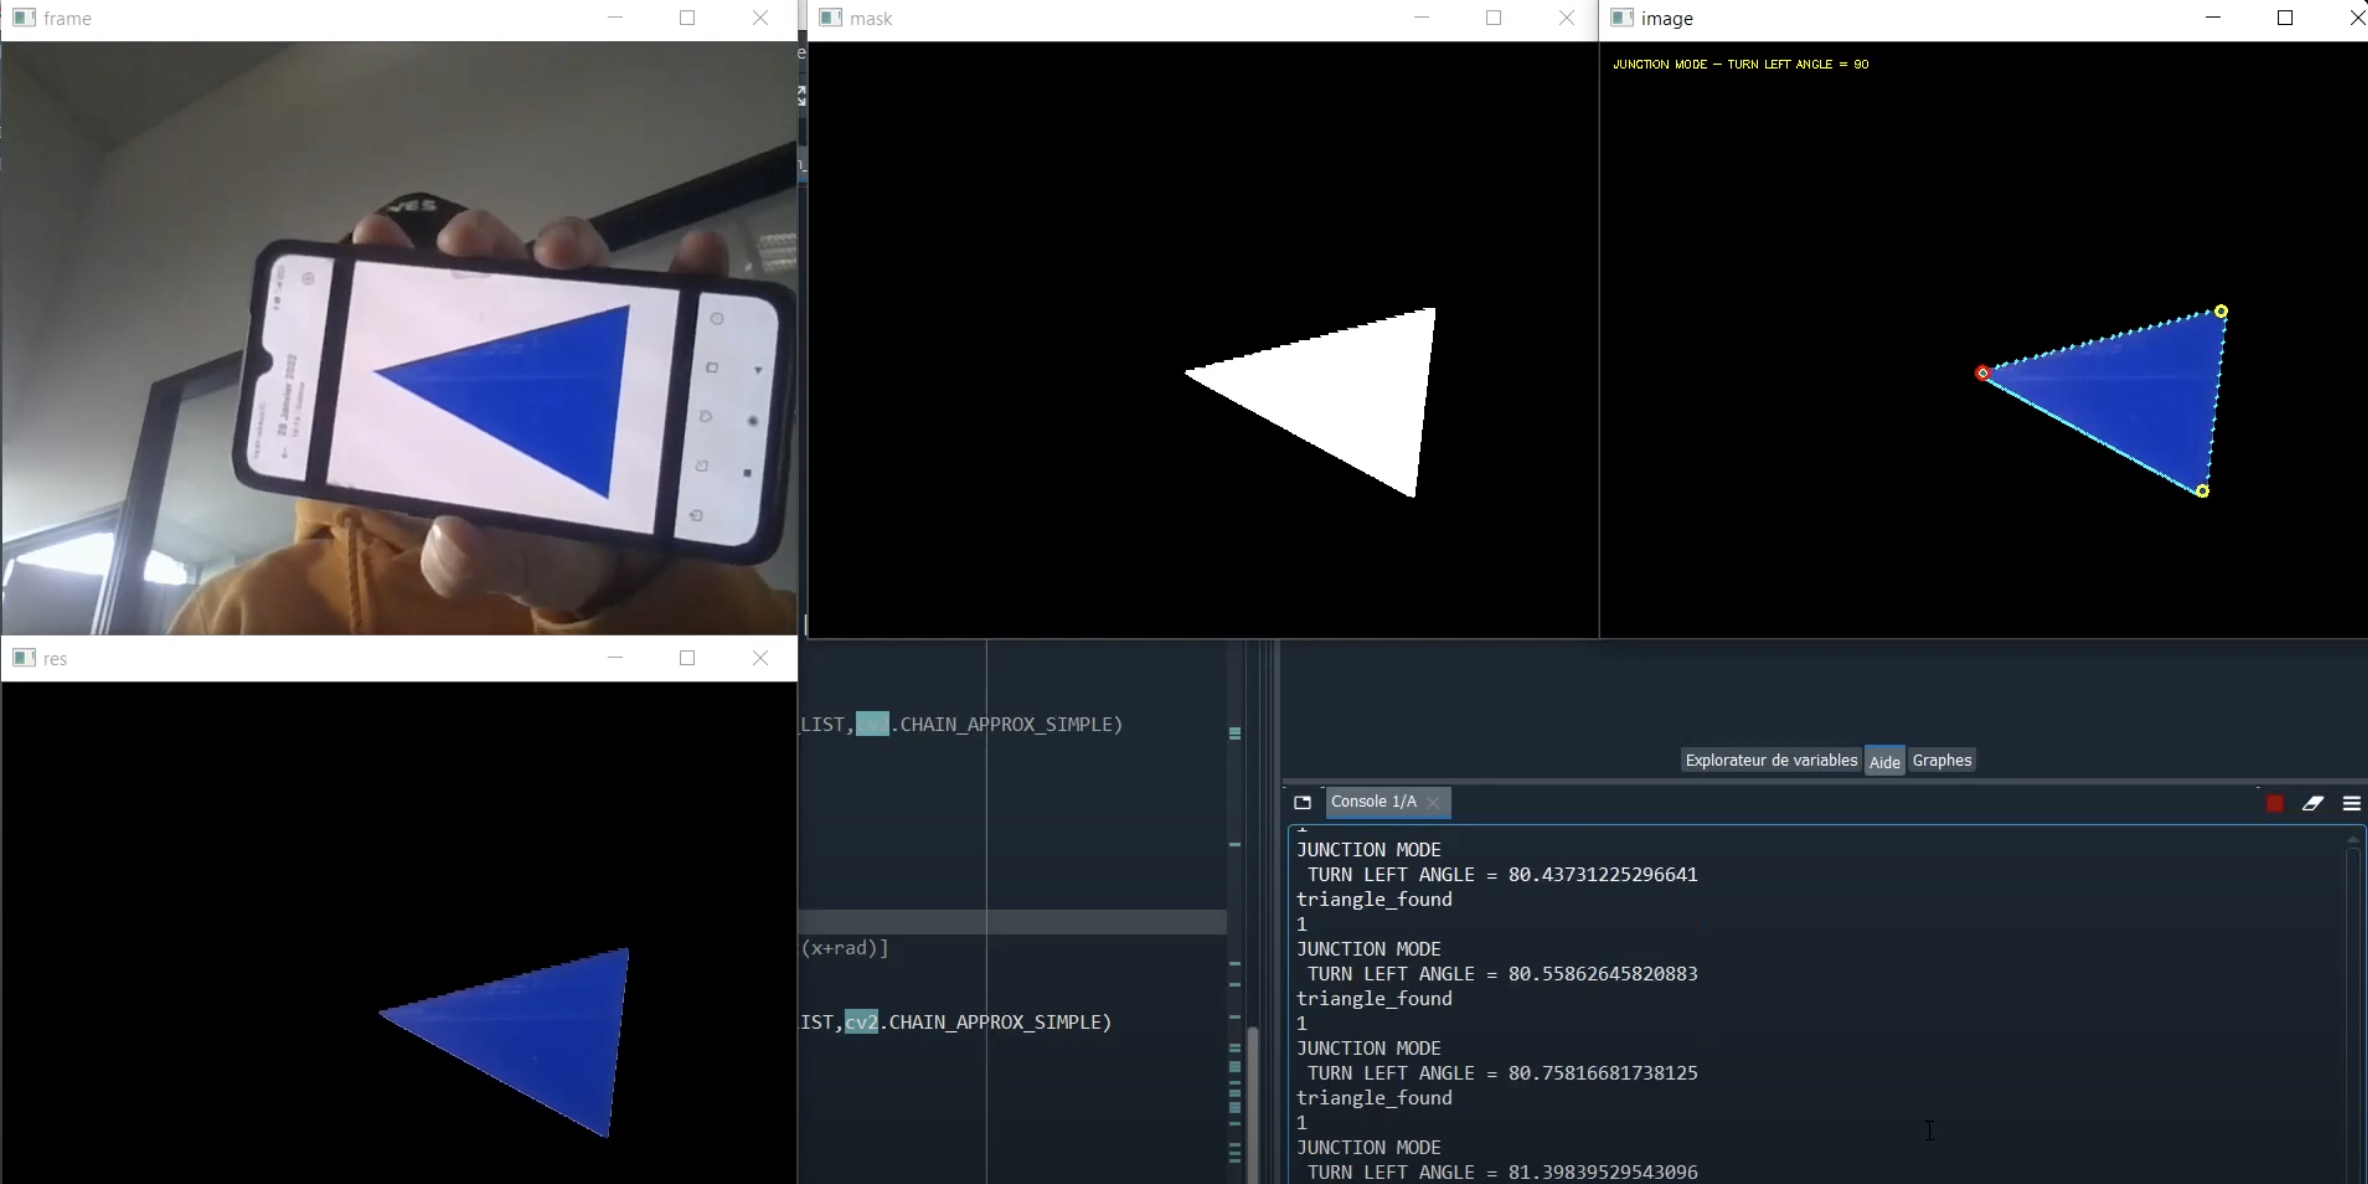
\includegraphics[width=0.5\textwidth]{assets/arrow-demo.png}}
    \caption{Demonstration of the arrow direction tracking solution \cite{b29}\cite{b30}.}
    \label{f9}
\end{figure}

\begin{figure}[htbp]
    \centerline{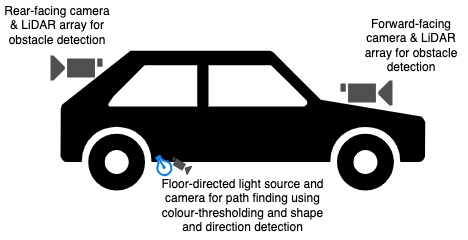
\includegraphics[width=0.5\textwidth]{assets/car-demo.png}}
    \caption{Diagram of autonomous trasportation system architecture.}
    \label{f10}
\end{figure}

The lane detection and tracking system, designed for the driver assistance system's vehicular lane monitoring functionality, will undergo adaptation to facilitate a line-following mechanism for the mobility scooter. This adaptation involves repurposing the lane detection algorithm to recognise and track specific tape shapes and colours affixed to the ground, interpreting these markings as navigational cues. At the beginning of a journey, the user can select a destination, thus setting the colour-masking threshold parameters to forward the correct shape colour. A camera positioned in a way pointing to the floor can detect the correct path of shapes since the colour-masking will ensure only the correct shape colour is passed into the frame, with surrounding pixels staying black. OpenCV simplifies the implementation of shape detection, as the work in \cite{b27} outlines an efficient method to achieve this using the Ramer-Douglas-Peucker contour approximation algorithm \cite{b28}. Derivation of the shape direction is possible by cropping to the region within the shape, isolating the isosceles triangle to detect the triangle's vertices outputs the direction, similar to the work in \cite{b29}\cite{b30}, demonstration in Figure \ref{f9}. A forward-facing camera with light detection and ranging (LiDAR) sensors enables the implementation of the simultaneous localisation and mapping (SLAM) method to detect obstacles, generate a map of the surroundings, and navigate to avoid obstructions when required to deviate from the tape-implemented path \cite{b31}\cite{b32}. Figure \ref{f10} shows the overall architecture involving this path detection and tracking system.

\subsubsection{Eye Blink and Gaze Control}
The earlier implemented eye blink and gaze detection system is pivotal in providing this system with user control and override functionalities. Gaze direction can potentially act as a means to alter the vehicle's direction or stop its movement. For example, a prolonged gaze or blinks in predefined patterns can signal a direction change or a halt.

\subsubsection{Retro-Fitting to Existing Vehicular System}
To achieve the required system modularity, the implementation of removable sensors and controls utilising magnetic components to attach to the metallic body of a vehicle, such as a mobility scooter. Creating a universal control interface ensures compatibility with different scooter models. A simplified and adaptable control interface would encompass steering, acceleration, and braking controls, allowing seamless integration with different vehicular systems. Servo implementation for controlling the vehicle's steering is perhaps the most difficult due to the size constraints and technical aspects of installing it onto a mobility scooter. A touch-screen with embedded speakers will be in front of the user for easy control of the system. There's a possibility to implement gaze and blink tracking to control the screen, thus controlling the system. Implementing user overrides for critical controls ensures safety, including accessible emergency stop buttons or switches that can instantly halt the scooter's autonomous operation, placing control back in the user's hands. Despite the universal control interface, preserving the original control surfaces, such as the accelerator, brake pedals and steering wheel, will ensure the means of a safe and natural user override.

\subsubsection{Interaction Modalities}
Discussing the interaction modalities provides a detailed summary of the whole system. Employing several interaction modalities can improve the safety of the user and the surrounding environment:

\begin{enumerate}[label=\alph*.]
    \item Tape-based navigational cues: Employ tape markings of distinct shapes and colours on the floor to indicate destinations. Different shape-color combinations depict various destinations; the orientation of arrow shapes shows the direction of travel. The user selects the destination, and the system follows the correct tape path using colour masking and shape recognition.
    \item Obstacle detection and navigation: The camera and LiDAR array with the SLAM method enable obstacle detection and mapping. The sensor array detects the surroundings to assemble a map and navigate around obstructions. With this method, the deviation from the tape-implemented path to avoid obstacles is possible.
    \item Blink and gaze control: Eye tracking can implement user control and override functionalities. The user's gaze or blinking pattern can signal direction changes or halts, allowing the user to influence the direction or overall control of the system.
    \item Physical controls: Implementation of a touch screen panel and preservation of the original vehicular control interfaces provide physical touch controls to the user. The user can interact with these surfaces to influence the direction and overall control of the system, including safety overrides.
\end{enumerate}

\subsection{Safety, Ethics, and Impact of System}
Incorporating safety features for accident prevention should be of utmost priority for any autonomous transportation system. Implementing a range of safety features and protocols is a must to mitigate potential risks and ensure accident prevention. All the discussion points on this aspect of the driver monitoring system apply here.

A constant and live metrics feed reporting the system's performance, location and route must be available to caregivers and shop floor assistants. This vigilance ensures proactive management and immediate intervention in case of deviations or unforeseen hazards to minimise the risk of accidents. There must be a kill switch to terminate the system at the press of a button, both in the vehicle accessible by the user and remotely accessible by the caregiver or shop floor assistant.

The system must emphasise intuitive user interfaces, employing readable fonts, clear icons and a friendly colour scheme to ensure ease of use. The system must focus on user-empowering design choices rather than those that intrude upon their independence, striking a balance between autonomy and assistance. It operates as a reliable aid, allowing users to navigate expansive structures with confidence and minimal external intervention, fostering a sense of self-reliance and dignity.

\section{Conclusion}

The convergence of machine vision and human-machine interaction yields a new era of support systems aiming to improve the lives of diverse populations facing various challenges. Mentions of driver assistance and autonomous transportation systems in this article represent significant strides in this domain, each catering to distinct yet intersecting needs.

The driver assistance system is a beacon of safety and assistance, offering invaluable aid to drivers in harsh conditions traversing complex roadways. Leveraging machine vision technologies, the system pioneers lane detection and tracking, promising heightened safety by tracking lane departures, driver fatigue and focus levels, generating quantitative and definitive scores to gauge both metrics. To enhance its efficacy further, continuous refinements in the lane detection algorithms and integration with more advanced sensor technologies like LiDAR could bolster its ability to detect and respond to dynamic environments, integrating the detection and tracking of other road users. Furthermore, positioning cameras in better locations, such as below the wing mirrors for lane markings capture, improves the system's immunity to varying environmental conditions.

On the other hand, the autonomous transportation system emerges as a revolutionary mobility aid, particularly beneficial to the vulnerable population when traversing intricate buildings. This system's marriage of machine vision and human-machine interaction leads to a refined architecture enabling tape-based navigational cues, obstacle detection, and user interaction through gaze and blink control. To augment its capabilities, ongoing improvements in obstacle detection algorithms, including machine learning methodologies, and the seamless integration of more robust safety overrides could fortify its reliability. Further advancements to emphasising modularity can amplify their universality and applicability across many vehicles and user scenarios.

The potential impact of these systems exceeds mere convenience, bringing to light a transformative shift in the lives of vulnerable populations by augmenting safety and fostering independence with assistance. Workers subjected to challenging environments may find relief through driver assistance, mitigating risks and ensuring safer work environments for all road users. The autonomous transportation system opens doors to unprecedented mobility, offering vulnerable populations a renewed sense of freedom and confidence in navigating complex spaces. Moreover, these systems alleviate the burdens on caregivers by providing dependable aids that reduce the constant need for supervision and assistance, redefining the relationship between caregivers and those under their care, and encouraging greater independence while ensuring safety and peace of mind.

\begin{thebibliography}{00}

    \bibitem{b1} "Lane departure warning system," Wikipedia, https://en.wikipedia.org/wiki/Lane\_departure\_warning\_system (accessed Dec. 27, 2023).

    \bibitem{b2} "Press corner," European Commission - European Commission, https://ec.europa.eu/commission/presscorner/detail/en/ip\_22\_4312 (accessed Dec. 27, 2023).

    \bibitem{b3} C. Y. Low, H. Zamzuri and S. A. Mazlan, "Simple robust road lane detection algorithm," 2014 5th International Conference on Intelligent and Advanced Systems (ICIAS), Kuala Lumpur, Malaysia, 2014, pp. 1-4, doi: 10.1109/ICIAS.2014.6869550.

    \bibitem{b4} L. Chandrasekar and G. Durga, "Implementation of Hough Transform for image processing applications," 2014 International Conference on Communication and Signal Processing, Melmaruvathur, India, 2014, pp. 843-847, doi: 10.1109/ICCSP.2014.6949962.

    \bibitem{b5} A. R, “Hough transforms in image processing,” Scaler Topics, https://www.scaler.com/topics/hough-transform-in-image-processing/ (accessed Dec. 28, 2023).

    \bibitem{b6} N. Vykari, “Understanding Hough Transform with a lane detection model,” Paperspace Blog, https://blog.paperspace.com/understanding-hough-transform-lane-detection/ (accessed Dec. 28, 2023).

    \bibitem{b7} T. Tasneem and Z. Afroze, "A New Method of Improving Performance of Canny Edge Detection," 2019 2nd International Conference on Innovation in Engineering and Technology (ICIET), Dhaka, Bangladesh, 2019, pp. 1-5, doi: 10.1109/ICIET48527.2019.9290676.

    \bibitem{b8} RideScapes, “ASMR highway driving at night (no talking, no music) - busan to Seoul, Korea,” YouTube, https://www.youtube.com/watch?v=nABR88G\_2cE (accessed Dec. 30, 2023).

    \bibitem{b9} A. Rosebrock, “Zero-parameter, automatic canny edge detection with python and opencv,” PyImageSearch, https://pyimagesearch.com/2015/04/06/zero-parameter-automatic-canny-edge-detection-with-python-and-opencv/ (accessed Dec. 30, 2023).

    \bibitem{b10} “Hough Line transform,” OpenCV, https://docs.opencv.org/3.4/d9 /db0/tutorial\_hough\_lines.html (accessed Dec. 30, 2023).

    \bibitem{b11} “Driver monitoring system,” Wikipedia, https://en.wikipedia.org/wiki/Driver\_monitoring\_system (accessed Jan. 3, 2024).

    \bibitem{b12} Council of European Union, Council regulation ({EU}) no 2019/2144, https://eur-lex.europa.eu/eli/reg/2019/2144/oj (accessed Jan. 3, 2024).

    \bibitem{b13} “Classes,” Dlib C++ Library, http://dlib.net/python/index.html (accessed Jan. 3, 2024).

    \bibitem{b14} “Trained 68-Point Facial Landmark Model,” Dlib C++ Library, http://dlib.net/files/shape\_predictor\_68\_face\_landmarks.dat.bz2 (accessed Jan. 3, 2024).

    \bibitem{b15} B. Yagyesh, “Eye blink detection with opencv, python, and dlib,” GeeksforGeeks, https://www.geeksforgeeks.org/eye-blink-detection-with-opencv-python-and-dlib/ (accessed Jan. 3, 2024).

    \bibitem{b16} “CV::Simpleblobdetector class reference,” OpenCV, https://docs.opencv.org/3.4/d0/d7a/classcv\_1\_1SimpleBlobDetector.html (accessed Jan. 3, 2024).

    \bibitem{b17} G. Malhotra, “Building a Prototype to Track Eye Gaze,” dissertation, 2023

    \bibitem{b18} G. Malhotra, “GagandeepMalhotra/Building-a-Prototype-to-Track-Eye-Gaze,” GitHub, https://github.com/GagandeepMalhotra/Building-a-Prototype-to-Track-Eye-Gaze (accessed Jan. 3, 2024).

    \bibitem{b19} MediaInfo, “How Audi's light digitization is pointing the way toward the future,” Audi MediaCenter, https://www.audi-mediacenter.com/en/press-releases/how-audis-light-digitization-is-pointing-the-way-toward-the-future-14624 (accessed Jan. 4, 2024).

    \bibitem{b20} M. Dillon, “White Noise vs. Brown noise: Which one is best for sleep?,” CNET, https://www.cnet.com/health/sleep/white-noise-vs-brown-noise-which-one-is-best-for-sleep/ (accessed Jan. 4, 2024).

    \bibitem{b21} Passport BMW, “How to perfume the interior of a BMW with Ambient Air Package,” BMW, https://www.passportbmw.com/blogs/846/uncategorized/how-to-perfume-the-interior-of-a-bmw-with-ambient-air-package/ (accessed Jan. 4, 2024).

    \bibitem{b22} J. Lyons, “Struggling to stay alert? 10 best scents for waking up,” WebMD, https://www.webmd.com/sleep-disorders/features/best-scents-for-waking-up (accessed Jan. 4, 2024).

    \bibitem{b23} J. B. Cicchino, “Effects of lane departure warning on police-reported crash rates,” Journal of Safety Research, vol. 66, pp. 61-70, May 2018. doi:10.1016/j.jsr.2018.05.006

    \bibitem{b24} M. F. Ani, S. R. Kamat, M. Fukumi, and N. A. Noh, “A Critical Review on Driver Fatigue Detection and Monitoring System,” International Journal of Road Safety, vol. 1, pp. 53-58, Nov. 2020.

    \bibitem{b25} T. Arakawa, “Trends and future prospects of the drowsiness detection and estimation technology,” Sensors, vol. 21, no. 23, p. 7921, Nov. 2021. doi:10.3390/s21237921

    \bibitem{b26} Seeing Machines Limited, Majority of UK road users believe new eye-tracking technology to check driver attentiveness could help improve road safety, but public awareness remains low, according to survey, https://www.prnewswire.com/apac/news-releases/majority-of-uk-road-users-believe-new-eye-tracking-technology-to-check-driver-attentiveness-could-help-improve-road-safety-but-public-awareness-remains-low-according-to-survey-301838223.html (accessed Jan. 4, 2024).

    \bibitem{b27} A. Rosebrock, “OPENCV shape detection,” PyImageSearch, https://pyimagesearch.com/2016/02/08/opencv-shape-detection/ (accessed Jan. 5, 2024).

    \bibitem{b28} “Ramer-Douglas-Peucker algorithm,” Wikipedia, https://w.wiki/3X7H (accessed Jan. 5, 2024).

    \bibitem{b29} H. I. Adikari, “HishanIndrajith/ArrowDirectionPythonOpenCV,” GitHub, https://github.com/HishanIndrajith/ArrowDirectionPythonOpenCV (accessed Jan. 5, 2024).

    \bibitem{b30} A. Sicius, “Arrow (triangle) orientation detection based on OpenCV Python,” YouTube, https://www.youtube.com/watch?v=zL6M0vYCr4s (accessed Jan. 5, 2024).

    \bibitem{b31} MathWorks, “What is SLAM (simultaneous localization and mapping) - matlab \& simulink,” What Is SLAM (Simultaneous Localization and Mapping) - MATLAB \& Simulink - MATLAB \& Simulink, https://uk.mathworks.com/discovery/slam.html (accessed Jan. 5, 2024).

    \bibitem{b32} M. Chghaf, S. Rodriguez, and A. E. Ouardi, “Camera, Lidar and multi-modal SLAM systems for Autonomous Ground Vehicles: A survey,” Journal of Intelligent \& Robotic Systems, vol. 105, no. 1, 2022. doi:10.1007/s10846-022-01582-8 

\end{thebibliography}

\appendix

\subsection{Lane Detection and Tracking Source Code}
\label{a1}
\lstinputlisting[caption={Source code for the lane detection and tracking implementation, submitted as lane.py}, captionpos=b, label={lst1}, language=Python, basicstyle=\tiny, showspaces=false, showstringspaces=false tabsize=1, breaklines=true]{code/lane.py}


\subsection{Gaze and Blink Detection and Tracking Source Code}
\label{a2}
\lstinputlisting[caption={Source code for the eye gaze and blink detection and tracking implementation, submitted as eyes.py}, captionpos=b, label={lst2}, language=Python, basicstyle=\tiny, showspaces=false, showstringspaces=false tabsize=1, breaklines=true]{code/eyes.py}

\subsection{Python Dependencies for Project}
\label{a3}
\lstinputlisting[caption={List of pip dependencies that require installing prior to running the Python implementation code, submitted as requirements.txt}, captionpos=b, label={lst3}, basicstyle=\tiny, showspaces=false, showstringspaces=false tabsize=1, breaklines=true]{code/requirements.txt}

\end{document}
